\documentclass[12pt]{article}
\usepackage[paperwidth=25cm,paperheight=17cm,margin=1.4cm]{geometry}
\usepackage[T1]{fontenc}
\usepackage[utf8]{inputenc}
\usepackage[magyar]{babel}
\usepackage{lmodern}
\usepackage{amsmath}
\usepackage{enumitem}
\usepackage{array}
\usepackage{tikz}
\usetikzlibrary{arrows.meta,decorations.pathmorphing}
\usepackage{pgfplots}
\pgfplotsset{compat=1.16}
\usepackage[most]{tcolorbox}

\pagestyle{empty}
\setlength{\parindent}{0pt}
\setlength{\parskip}{4pt}
\setlist[itemize]{leftmargin=1.4em, itemsep=3pt, topsep=2pt, parsep=0pt}

\newcommand{\dia}[1]{\newpage{\Large\bfseries #1}\par\vspace{2pt}{\color{blue!50!black}\hrule height 1pt}\vspace{8pt}}

\newtcolorbox{pelda}[1][]{colback=green!4,colframe=green!45!black,fonttitle=\bfseries,
  title=Kidolgozott példa,left=5pt,right=5pt,top=3pt,bottom=3pt,before skip=6pt,after skip=4pt,#1}
\newtcolorbox{fontos}[1][]{colback=blue!3,colframe=blue!45!black,
  left=5pt,right=5pt,top=3pt,bottom=3pt,before skip=6pt,after skip=4pt,#1}

% egyenként érkező elektronok becsapódásai: #1 = próbálkozások száma, #2 = mag, #3 = felirat
\newcommand{\elektronpanel}[3]{%
  \begin{tikzpicture}
    \fill[black!4] (-1.9,0) rectangle (1.9,1.9);
    \pgfmathsetseed{#2}
    \foreach \i in {1,...,#1}{
      \pgfmathsetmacro{\x}{1.9*rand}
      \pgfmathsetmacro{\y}{1.9*rnd}
      \pgfmathsetmacro{\p}{cos(300*\x)*cos(300*\x)*exp(-\x*\x/1.1)}
      \pgfmathsetmacro{\u}{rnd}
      \ifdim \u pt < \p pt \fill (\x,\y) circle (0.5pt); \fi
    }
    \draw (-1.9,0) rectangle (1.9,1.9);
    \node[below] at (0,0) {\small #3};
  \end{tikzpicture}}

\begin{document}

%====================================================================
\begin{center}
  \vspace*{1.2cm}
  {\Huge\bfseries Mi a fény?}\\[8pt]
  {\Large A fény kettős természete}\\[1.4cm]
\end{center}

\begin{center}
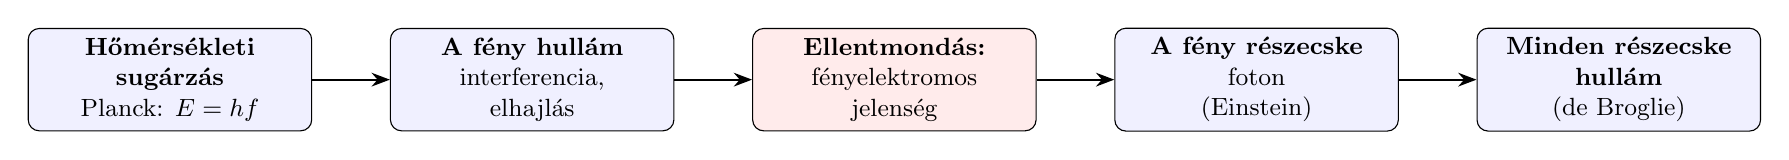
\begin{tikzpicture}[font=\small,
    allomas/.style={draw,rounded corners,fill=blue!6,minimum width=3.6cm,minimum height=1.3cm,align=center},
    >=Stealth]
  \node[allomas] (a) at (0,0)    {\textbf{Hőmérsékleti}\\\textbf{sugárzás}\\Planck: $E = hf$};
  \node[allomas] (b) at (4.6,0)  {\textbf{A fény hullám}\\interferencia,\\elhajlás};
  \node[allomas,fill=red!8] (c) at (9.2,0) {\textbf{Ellentmondás:}\\fényelektromos\\jelenség};
  \node[allomas] (d) at (13.8,0) {\textbf{A fény részecske}\\foton\\(Einstein)};
  \node[allomas] (e) at (18.4,0) {\textbf{Minden részecske}\\\textbf{hullám}\\(de Broglie)};
  \foreach \u/\v in {a/b,b/c,c/d,d/e} \draw[->,thick] (\u) -- (\v);
\end{tikzpicture}
\end{center}

\vspace{1.2cm}
\begin{center}
\fbox{\parbox{0.9\textwidth}{\centering
  $h = 6{,}63\cdot 10^{-34}~\text{J}\cdot\text{s}$, \quad
  $c = 3\cdot 10^{8}~\tfrac{\text{m}}{\text{s}}$, \quad
  $e = 1{,}6\cdot 10^{-19}~\text{C}$, \quad
  $m_e = 9{,}1\cdot 10^{-31}~\text{kg}$, \quad
  $1~\text{eV} = 1{,}6\cdot 10^{-19}~\text{J}$}}
\end{center}

%====================================================================
\dia{1. Hőmérsékleti sugárzás -- minden test világít}

\begin{minipage}[t]{0.56\linewidth}\vspace{0pt}
\begin{itemize}
  \item Minden test elektromágneses sugárzást bocsát ki, amelynek spektruma a test
    \textbf{hőmérsékletétől} függ. Szobahőmérsékleten ez infravörös, ezért nem látjuk.
  \item Melegebb testnél a spektrum csúcsa a \textbf{rövidebb hullámhosszak} felé tolódik:
    a hevített vas sötétvörös $\to$ narancs $\to$ fehér izzású lesz.
    \[ \textbf{Wien-féle eltolódási törvény:}\quad
       \lambda_\text{max}\cdot T = 2{,}9\cdot 10^{-3}~\text{m}\cdot\text{K} \]
  \item A kisugárzott teljes teljesítmény (a görbe alatti terület) meredeken nő:
    $P \propto T^4$ (Stefan--Boltzmann-törvény). Kétszeres hőmérséklet $\to$ 16-szoros
    teljesítmény.
\end{itemize}
\end{minipage}\hfill
\begin{minipage}[t]{0.42\linewidth}\vspace{0pt}\centering
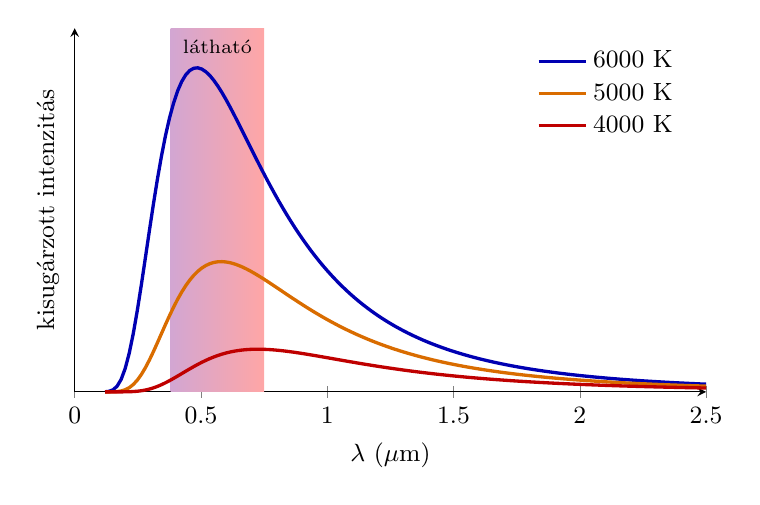
\begin{tikzpicture}
\begin{axis}[width=9.6cm,height=6.2cm,xmin=0,xmax=2.5,ymin=0,ymax=0.3,
    xlabel={$\lambda$ ($\mu$m)},ylabel={kisugárzott intenzitás},
    yticklabels={},ytick=\empty,xtick={0,0.5,1,1.5,2,2.5},
    tick label style={font=\small},label style={font=\small},
    axis lines=left,clip=false,
    legend style={font=\small,draw=none,fill=none,at={(0.97,0.97)},anchor=north east}]
  \fill[left color=violet!35,right color=red!35] (axis cs:0.38,0) rectangle (axis cs:0.75,0.3);
  \node[font=\scriptsize] at (axis cs:0.565,0.285) {látható};
  \addplot[very thick,blue!70!black,domain=0.12:2.5,samples=150]
    {1/(x^5*(exp(14388/(x*6000))-1))};
  \addplot[very thick,orange!85!black,domain=0.12:2.5,samples=150]
    {1/(x^5*(exp(14388/(x*5000))-1))};
  \addplot[very thick,red!75!black,domain=0.12:2.5,samples=150]
    {1/(x^5*(exp(14388/(x*4000))-1))};
  \legend{$6000$~K,$5000$~K,$4000$~K}
\end{axis}
\end{tikzpicture}
\end{minipage}

\vspace{4pt}
\begin{center}
\renewcommand{\arraystretch}{1.3}
\begin{tabular}{|l|c|c|l|}
\hline
\textbf{Test} & $\boldsymbol{T}$ & $\boldsymbol{\lambda_\text{max}}$ & \textbf{Következmény} \\ \hline
Nap felszíne & $5800$~K & $500$~nm & a látható tartomány közepe -- szemünk erre ,,hangolódott'' \\
izzólámpa szála & $2800$~K & $1{,}04~\mu$m & infravörös! Csak néhány \% látható fény $\to$ rossz hatásfok \\
emberi test & $310$~K & $9{,}4~\mu$m & távoli infravörös -- ezt látja a hőkamera \\ \hline
\end{tabular}
\end{center}

%====================================================================
\dia{2. Planck ötlete: az energia adagokban jön}

\begin{itemize}
  \item A klasszikus fizika a sugárzási görbe alakját nem tudta megmagyarázni: rövid
    hullámhosszakon végtelen nagy sugárzást jósolt (,,ultraibolya katasztrófa'').
  \item \textbf{Planck (1900):} a görbe pontosan kijön, ha feltesszük, hogy a test az
    energiát csak meghatározott adagokban, \textbf{kvantumokban} bocsáthatja ki és nyelheti el:
\end{itemize}

\begin{fontos}
\[ E = hf = \frac{hc}{\lambda}, \qquad h = 6{,}63\cdot 10^{-34}~\text{J}\cdot\text{s}
   \quad (\text{Planck-állandó}) \]
\centering Nagyobb frekvencia (rövidebb hullámhossz) $\Rightarrow$ nagyobb energiájú kvantum.
Planck maga is csak matematikai ,,trükknek'' tartotta.
\end{fontos}

\begin{itemize}
  \item \textbf{Elektronvolt:} az az energia, amelyet egy elektron $1$~V feszültségen
    áthaladva nyer: $1~\text{eV} = 1{,}6\cdot 10^{-19}~\text{J}$. Hasznos rövidítés:
    $hc \approx 1240~\text{eV}\cdot\text{nm}$, vagyis $E\,[\text{eV}] \approx
    \dfrac{1240}{\lambda\,[\text{nm}]}$.
\end{itemize}

\begin{pelda}
\textbf{Vörös fény} ($700$~nm): $\;E = \dfrac{6{,}63\cdot 10^{-34}\cdot 3\cdot 10^8}{7\cdot 10^{-7}}~\text{J}
  \approx 2{,}84\cdot 10^{-19}~\text{J} \approx 1{,}8~\text{eV}$. \qquad
\textbf{Ibolya fény} ($400$~nm): $\;E \approx 4{,}97\cdot 10^{-19}~\text{J} \approx 3{,}1~\text{eV}$.\\[3pt]
Egy kvantum energiája nagyon kicsi: egy $1$~mW-os vörös lézermutató másodpercenként
$\dfrac{10^{-3}~\text{J}}{2{,}84\cdot 10^{-19}~\text{J}} \approx 3{,}5\cdot 10^{15}$ kvantumot bocsát ki.
Ezért nem vesszük észre a hétköznapokban az adagosságot.
\end{pelda}

%====================================================================
\dia{3. A fény hullám: interferencia és elhajlás}

\begin{minipage}[t]{0.58\linewidth}\vspace{0pt}
\begin{itemize}
  \item A fény \textbf{elektromágneses hullám} (Maxwell, 1865): $c = \lambda f$, a látható
    tartomány $380$--$750$~nm.
  \item Hullámjelenségek: \textbf{interferencia}, \textbf{elhajlás}, \textbf{polarizáció}
    (ez utóbbi azt mutatja, hogy a fény transzverzális hullám).
  \item \textbf{Young kétréses kísérlete (1801):} két keskeny résen átjutó fény az ernyőn
    fényes és sötét csíkokat hoz létre. Ahol a két résből érkező hullámok útkülönbsége
    $k\lambda$, ott erősítik, ahol $(k+\tfrac12)\lambda$, ott kioltják egymást.
  \item \textbf{Optikai rács:} sok, egymástól $d$ távolságra lévő rés ($d$ a rácsállandó).
    Éles, fényes foltok ott, ahol
    \[ d\sin\alpha_k = k\lambda, \qquad k = 0, \pm1, \pm2, \dots \]
    Fehér fénynél színkép jön létre: a vörös hajlik el jobban, mint az ibolya.
\end{itemize}
\end{minipage}\hfill
\begin{minipage}[t]{0.40\linewidth}\vspace{0pt}\centering
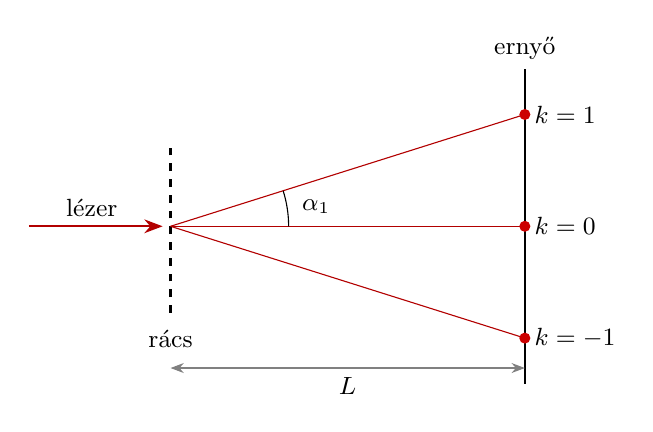
\begin{tikzpicture}[scale=1.0,>=Stealth]
  \draw[->,thick,red!70!black] (-1.8,0) -- (-0.1,0);
  \node[above,font=\small] at (-1,0) {lézer};
  \foreach \y in {-1.1,-0.9,...,1.1} \draw[thick] (0,\y) -- (0,\y+0.1);
  \node[below,font=\small] at (0,-1.2) {rács};
  \draw[thick] (4.5,-2.0) -- (4.5,2.0);
  \node[above,font=\small] at (4.5,2.0) {ernyő};
  \draw[red!70!black] (0,0) -- (4.5,0);
  \draw[red!70!black] (0,0) -- (4.5,1.42);
  \draw[red!70!black] (0,0) -- (4.5,-1.42);
  \foreach \y/\k in {0/0,1.42/1,-1.42/-1}
    \fill[red!80!black] (4.5,\y) circle (2pt) node[right,black,font=\small] {$k=\k$};
  \draw (1.5,0) arc (0:17.5:1.5);
  \node[font=\small] at (1.85,0.25) {$\alpha_1$};
  \draw[<->,gray] (0,-1.8) -- node[below,font=\small,black] {$L$} (4.5,-1.8);
\end{tikzpicture}
\end{minipage}

\begin{fontos}
\centering\textbf{Fény $+$ fény $=$ sötétség.} Ezt csak hullámok tudják: részecskékből több
résen át mindenhová csak \emph{több} érkezhetne. Az interferencia a hullámtermészet
legerősebb bizonyítéka.
\end{fontos}

%====================================================================
\dia{4. Kidolgozott példa: lézermutató és CD}

\begin{pelda}
Egy CD lemez sávjai optikai rácsként működnek, a sávtávolság $d = 1{,}6~\mu\text{m}$. Vörös
lézermutatóval ($\lambda = 650$~nm) világítjuk meg, a fal $L = 0{,}5$~m-re van.

\medskip
\textbf{Első rend:} $\sin\alpha_1 = \dfrac{\lambda}{d} = \dfrac{0{,}65}{1{,}6} \approx 0{,}406
  \;\Rightarrow\; \alpha_1 \approx 24{,}0^\circ$, \quad a falon $x_1 = L\tan\alpha_1 \approx 0{,}22$~m.

\textbf{Második rend:} $\sin\alpha_2 = \dfrac{2\lambda}{d} \approx 0{,}81 \;\Rightarrow\;
  \alpha_2 \approx 54{,}3^\circ$, \quad $x_2 = L\tan\alpha_2 \approx 0{,}70$~m.

\textbf{Hány folt?} $\sin\alpha \le 1 \Rightarrow k \le d/\lambda \approx 2{,}46$, tehát
$k_\text{max} = 2$: összesen $5$ folt ($k = 0, \pm1, \pm2$).
\end{pelda}

\begin{fontos}[colback=red!4,colframe=red!55!black]
\textbf{Gyakori hiba:} a kis szögekre érvényes $x \approx k\lambda L/d$ közelítés itt
$0{,}20$ és $0{,}41$~m-t adna. A második rendnél ez teljesen rossz: nagy szögeknél
mindig $\sin$ és $\tan$ kell.
\end{fontos}

\begin{itemize}
  \item DVD-vel ($d = 0{,}74~\mu$m) csak az első rend látszik, kb.\ $61^\circ$-nál.
  \item Fehér fényben a CD azért szivárványos, mert minden hullámhossz más szögben
    hajlik el.
\end{itemize}

%====================================================================
\dia{5. Ami nem fér bele a hullámképbe: a fényelektromos jelenség}

\begin{minipage}[t]{0.68\linewidth}\vspace{0pt}
\textbf{Hallwachs kísérlete (1888):} negatívra töltött cinklemezt elektroszkópra teszünk.
\begin{itemize}
  \item Ultraibolya fénnyel megvilágítva az elektroszkóp \textbf{kisül}: a fény
    elektronokat lök ki a fémből. Ez a \textbf{fényelektromos jelenség} (fotoeffektus).
  \item Látható fénnyel -- \emph{akármilyen erős lámpával} -- \textbf{nem sül ki}.
  \item Pozitív lemeznél UV-vel sem sül ki: a kilépő részecskék negatívak (elektronok),
    és a pozitív lemez visszavonzza őket.
\end{itemize}
\end{minipage}\hfill
\begin{minipage}[t]{0.28\linewidth}\vspace{0pt}\centering
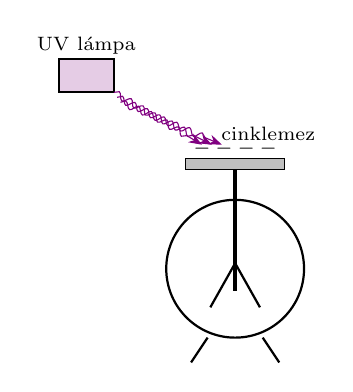
\begin{tikzpicture}[scale=0.7,>=Stealth]
  \draw[thick] (0,-0.2) circle (1.25);
  \draw[very thick] (0,1.6) -- (0,-0.6);
  \draw[thick] (0,-0.1) -- (-0.45,-0.9);
  \draw[thick] (0,-0.1) -- (0.45,-0.9);
  \fill[gray!50] (-0.9,1.6) rectangle (0.9,1.8);
  \draw (-0.9,1.6) rectangle (0.9,1.8);
  \node[above,font=\scriptsize] at (0.6,1.95) {cinklemez};
  \foreach \x in {-0.6,-0.2,0.2,0.6} \node[font=\scriptsize] at (\x,1.97) {$-$};
  \draw[thick] (-0.5,-1.45) -- (-0.8,-1.9);
  \draw[thick] (0.5,-1.45) -- (0.8,-1.9);
  \draw[thick,fill=violet!20] (-3.2,3.0) rectangle (-2.2,3.6);
  \node[font=\scriptsize] at (-2.7,3.85) {UV lámpa};
  \foreach \d in {0,0.3,0.6}
    \draw[->,violet,decorate,decoration={snake,amplitude=1.2pt,segment length=5pt,post length=2mm}]
      (-2.2+\d*0.2,3.0-\d*0.3) -- (-0.6+\d*0.6,2.05);
\end{tikzpicture}
\end{minipage}

\vspace{6pt}
\begin{center}
\renewcommand{\arraystretch}{1.45}
\begin{tabular}{|>{\raggedright\arraybackslash}p{5.2cm}|>{\raggedright\arraybackslash}p{6.6cm}|>{\raggedright\arraybackslash}p{8.2cm}|}
\hline
\textbf{Kérdés} & \textbf{A hullámelmélet szerint\dots} & \textbf{A mérések szerint\dots} \\ \hline
Kell-e egy minimális frekvencia? & nem: elég erős fény bármilyen színnel működne
  & \textbf{igen:} egy \textbf{határfrekvencia} ($f_0$) alatt semmilyen intenzitással nincs kilépés \\ \hline
Mitől függ az elektronok legnagyobb mozgási energiája? & az intenzitástól (erősebb hullám,
  nagyobb ,,lökés'') & \textbf{csak a frekvenciától}; az intenzitás csak a kilépő
  elektronok \emph{számát} növeli \\ \hline
Van-e késés? & gyenge fénynél idő kell, amíg az elektron ,,összegyűjti'' az energiát
  & \textbf{nincs:} a kilépés azonnal megindul \\ \hline
\end{tabular}
\end{center}

%====================================================================
\dia{6. Einstein magyarázata (1905): a fény fotonokból áll}

\begin{minipage}[t]{0.62\linewidth}\vspace{0pt}
\begin{itemize}
  \item Nemcsak a kibocsátás adagos: maga a fény is részecskékből, \textbf{fotonokból}
    áll. Egy foton energiája $E = hf$.
  \item Egy foton \textbf{egyetlen elektronnak} adja át a teljes energiáját, és közben
    elnyelődik. Két foton energiája nem adódik össze egy elektronon.
  \item Az elektronnak a kilépéshez legalább a \textbf{kilépési munkát} ($W_\text{ki}$, a
    fémre jellemző) kell legyőznie. A maradék lesz a mozgási energiája:
\end{itemize}
\begin{fontos}
\[ hf = W_\text{ki} + \tfrac12 m v_\text{max}^2 \qquad\qquad
   f_0 = \frac{W_\text{ki}}{h}, \quad \lambda_0 = \frac{hc}{W_\text{ki}} \]
\end{fontos}
\end{minipage}\hfill
\begin{minipage}[t]{0.35\linewidth}\vspace{0pt}\centering
\renewcommand{\arraystretch}{1.3}
\begin{tabular}{|l|c|c|}
\hline
\textbf{Fém} & $\boldsymbol{W_\text{ki}}$ & $\boldsymbol{\lambda_0}$ \\ \hline
cézium & $2{,}1$~eV & $590$~nm \\
nátrium & $2{,}3$~eV & $540$~nm \\
cink & $4{,}3$~eV & $290$~nm \\ \hline
\end{tabular}

\medskip
{\small A cink határhullámhossza az ultraibolyában van: ezért működött Hallwachs
kísérlete csak UV-fénnyel.}
\end{minipage}

\vspace{4pt}
\textbf{Mindhárom megfigyelés megmagyarázható:}
\begin{itemize}
  \item \textbf{Határfrekvencia:} ha $hf < W_\text{ki}$, egyetlen foton sem tud elektront
    kiszakítani, akárhány érkezik is.
  \item \textbf{A mozgási energia csak $f$-től függ:} $\tfrac12 mv_\text{max}^2 = hf -
    W_\text{ki}$. Az \textbf{intenzitás a fotonok számát} adja meg: erősebb fény $\to$
    több foton $\to$ több elektron (nagyobb áram), de nem gyorsabbak.
  \item \textbf{Nincs késés:} az elektron egy egész fotont egyszerre nyel el, nem kell
    energiát gyűjtenie.
\end{itemize}
{\small Einstein 1921-ben ezért kapott Nobel-díjat, nem a relativitáselméletért.}

%====================================================================
\dia{7. Fotocella és zárófeszültség -- Millikan mérése}

\begin{minipage}[t]{0.55\linewidth}\vspace{0pt}
\begin{itemize}
  \item \textbf{Fotocella:} vákuumcső, benne a megvilágított fém (\textbf{katód}) és egy
    gyűjtőelektróda (\textbf{anód}). Az anódra jutó elektronok áramot (fotoáramot) hoznak
    létre.
  \item Ha az anódot negatívra kapcsoljuk, a tér fékezi az elektronokat. A
    \textbf{zárófeszültségnél} ($U_\text{z}$) már a leggyorsabbak sem jutnak át, az
    áram megszűnik:
    \[ eU_\text{z} = \tfrac12 m v_\text{max}^2 \]
    Voltban mérve $U_\text{z}$ éppen a legnagyobb mozgási energia eV-ban.
  \item Einstein egyenletéből:
    $\;U_\text{z} = \dfrac{h}{e}\,f - \dfrac{W_\text{ki}}{e}$, vagyis \textbf{egyenes}:
    \begin{itemize}
      \item meredeksége $h/e$, \textbf{minden fémre ugyanaz};
      \item az $f$ tengelyt a határfrekvenciánál ($f_0$) metszi;
      \item más fém: \textbf{párhuzamos} egyenes, eltolva;
      \item erősebb fény: \textbf{ugyanaz} az egyenes (csak az áram nő).
    \end{itemize}
  \item \textbf{Millikan (1916)} meg akarta cáfolni Einsteint. Mérése ehelyett igazolta az
    egyenletet, és pontosan kimérte $h$ értékét.
\end{itemize}
\end{minipage}\hfill
\begin{minipage}[t]{0.42\linewidth}\vspace{0pt}\centering
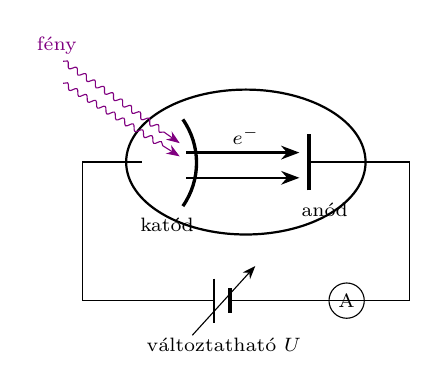
\begin{tikzpicture}[scale=0.8,>=Stealth,font=\small]
  % cső
  \draw[thick] (0,0) ellipse (1.9 and 1.15);
  \draw[very thick] (-1.0,-0.7) arc (-35:35:1.2);
  \node[font=\scriptsize] at (-1.25,-1.0) {katód};
  \draw[very thick] (1.0,-0.45) -- (1.0,0.45);
  \node[font=\scriptsize] at (1.25,-0.75) {anód};
  \foreach \y in {-0.25,0.15}
    \draw[->,thick] (-0.95,\y) -- (0.85,\y);
  \node[font=\scriptsize] at (0,0.42) {$e^-$};
  \foreach \d in {0,0.35}
    \draw[->,violet,decorate,decoration={snake,amplitude=1pt,segment length=4pt,post length=2mm}]
      (-2.9,1.6-\d) -- (-1.05,0.3-\d*0.6);
  \node[violet,font=\scriptsize] at (-3.0,1.85) {fény};
  % áramkör
  \draw (-0.75,0) -- (-0.75,0);
  \draw (-1.65,0) -- (-2.6,0) -- (-2.6,-2.2) -- (-0.5,-2.2);
  \draw (0.5,-2.2) -- (2.6,-2.2) -- (2.6,0) -- (1.0,0);
  \draw[thick] (-0.5,-1.85) -- (-0.5,-2.55);
  \draw[very thick] (-0.25,-2.0) -- (-0.25,-2.4);
  \draw[->] (-0.85,-2.75) -- (0.15,-1.65);
  \draw (-0.25,-2.2) -- (0.5,-2.2);
  \node[font=\scriptsize] at (-0.35,-2.9) {változtatható $U$};
  \draw (1.6,-2.2) circle (0.28) node {\scriptsize A};
  \fill[white] (1.32,-2.2) rectangle (1.88,-2.2);
\end{tikzpicture}

\vspace{4pt}
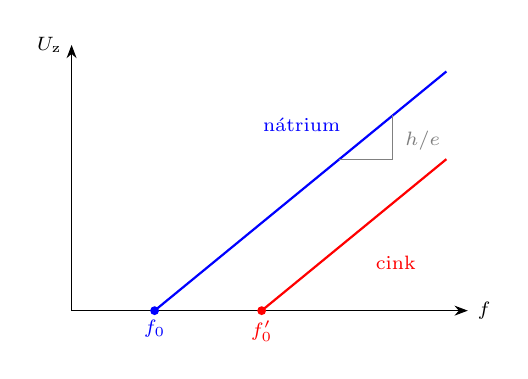
\begin{tikzpicture}[x=0.68cm,y=1.35cm,>=Stealth]
  \draw[->] (0,0) -- (7.4,0) node[right] {\scriptsize $f$};
  \draw[->] (0,0) -- (0,2.5) node[left] {\scriptsize $U_\text{z}$};
  \draw[thick,blue] (1.55,0) -- (7,2.25);
  \draw[thick,red] (3.55,0) -- (7,1.425);
  \fill[blue] (1.55,0) circle (1.6pt) node[below,font=\scriptsize] {$f_0$};
  \fill[red] (3.55,0) circle (1.6pt) node[below,font=\scriptsize] {$f_0'$};
  \node[blue,font=\scriptsize,anchor=east] at (5.2,1.75) {nátrium};
  \node[red,font=\scriptsize,anchor=west] at (5.5,0.45) {cink};
  \draw[gray] (5,1.426) -- (6,1.426) -- (6,1.84);
  \node[gray,font=\scriptsize,anchor=west] at (6.05,1.6) {$h/e$};
\end{tikzpicture}
\end{minipage}

%====================================================================
\dia{8. Kidolgozott példa: cinklemez UV-fényben}

\begin{pelda}
Cinklemezt ($W_\text{ki} = 4{,}3$~eV) $200$~nm-es ultraibolya fénnyel világítunk meg.

\medskip
\textbf{A foton energiája:} $\;E = \dfrac{hc}{\lambda} = \dfrac{1240~\text{eV}\cdot\text{nm}}{200~\text{nm}}
  = 6{,}2~\text{eV}$ \quad ($\approx 9{,}9\cdot 10^{-19}$~J).

\textbf{Legnagyobb mozgási energia:} $\;\tfrac12 mv_\text{max}^2 = hf - W_\text{ki} =
  6{,}2 - 4{,}3 = 1{,}9~\text{eV}$, \quad tehát a zárófeszültség $U_\text{z} = 1{,}9$~V.

\textbf{Legnagyobb sebesség} (az energiát \emph{joule-ba} kell váltani!):
\[ v_\text{max} = \sqrt{\frac{2\cdot 1{,}9\cdot 1{,}6\cdot 10^{-19}~\text{J}}{9{,}1\cdot 10^{-31}~\text{kg}}}
   \approx 8{,}2\cdot 10^{5}~\frac{\text{m}}{\text{s}} \]

\textbf{Határhullámhossz:} $\;\lambda_0 = \dfrac{1240~\text{eV}\cdot\text{nm}}{4{,}3~\text{eV}}
  \approx 290~\text{nm}$. A látható fény fotonjai ($\le 3{,}3$~eV) gyengék ehhez.

\textbf{Kétszer erősebb UV-lámpával:} kétszer annyi foton $\to$ kétszeres fotoáram, de
$U_\text{z}$ és $v_\text{max}$ \emph{nem változik}.
\end{pelda}

%====================================================================
\dia{9. A foton: részecske, amelynek hullámhossza van}

\begin{minipage}[t]{0.60\linewidth}\vspace{0pt}
\begin{itemize}
  \item A foton energiája $E = hf$, lendülete
    \[ p = \frac{E}{c} = \frac{h}{\lambda}. \]
    Nincs nyugalmi tömege, mindig $c$ sebességgel mozog.
  \item \textbf{Compton-jelenség (1923):} elektronokon szóródó röntgensugárzás hullámhossza
    megnő. A foton és az elektron úgy ütközik, mint két golyó: az energia és a lendület is
    megmarad. A foton energiát ad át, ezért nő a hullámhossza.
  \item A fény lendülete nyomást fejt ki (fénynyomás): ezen alapul a napvitorla.
\end{itemize}
\end{minipage}\hfill
\begin{minipage}[t]{0.37\linewidth}\vspace{0pt}\centering
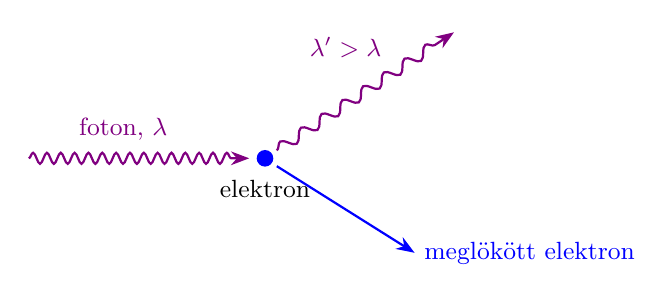
\begin{tikzpicture}[>=Stealth,font=\small]
  \draw[->,violet,thick,decorate,decoration={snake,amplitude=2pt,segment length=5pt,post length=2mm}]
    (-3,0) -- (-0.2,0);
  \node[violet,above] at (-1.8,0.1) {foton, $\lambda$};
  \fill[blue] (0,0) circle (3pt);
  \node[below] at (0,-0.15) {elektron};
  \draw[->,violet,thick,decorate,decoration={snake,amplitude=2pt,segment length=9pt,post length=2mm}]
    (0.15,0.1) -- (2.4,1.6);
  \node[violet,above left] at (1.6,1.15) {$\lambda' > \lambda$};
  \draw[->,blue,thick] (0.15,-0.1) -- (1.9,-1.2);
  \node[blue,right] at (1.9,-1.2) {meglökött elektron};
\end{tikzpicture}
\end{minipage}

\vspace{6pt}
\textbf{A fény kettős természete:}
\begin{center}
\renewcommand{\arraystretch}{1.45}
\begin{tabular}{|>{\raggedright\arraybackslash}p{10cm}|>{\raggedright\arraybackslash}p{10cm}|}
\hline
\textbf{Hullámtermészet} -- a fény \emph{terjedésében} &
\textbf{Részecsketermészet} -- a fény és az anyag \emph{kölcsönhatásában} \\ \hline
interferencia, elhajlás, polarizáció &
hőmérsékleti sugárzás (adagos kibocsátás), fényelektromos jelenség, Compton-jelenség \\ \hline
\end{tabular}
\end{center}
A fény nem ,,hol hullám, hol részecske'': \textbf{egyik klasszikus kép sem írja le
teljesen}. Mindkettő ugyanannak a kvantumos objektumnak egy-egy arca.

%====================================================================
\dia{10. De Broglie (1924): minden részecske hullám}

\begin{minipage}[t]{0.58\linewidth}\vspace{0pt}
\begin{itemize}
  \item Ha a hullámnak (fény) van részecsketermészete, akkor a részecskéknek (elektron,
    proton, atom\dots) is van hullámtermészete. A \textbf{de Broglie-hullámhossz}:
\end{itemize}
\begin{fontos}
\[ \lambda = \frac{h}{p} = \frac{h}{mv}, \qquad
   \text{$U$ feszültséggel gyorsított elektronra: } \lambda = \frac{h}{\sqrt{2meU}} \]
\end{fontos}
\begin{itemize}
  \item \textbf{Davisson és Germer (1927):} kristályra lőtt elektronok elhajlási képet adnak.
    A kristály atomjai rácsként működnek: ez a hullámtermészet kísérleti bizonyítéka.
  \item \textbf{Alkalmazás: elektronmikroszkóp.} A mikroszkóp a hullámhossznál kisebb
    részleteket nem tud felbontani. Fénnyel ez kb.\ $200$~nm, elektronokkal akár egyes
    atomok is láthatók.
\end{itemize}
\end{minipage}\hfill
\begin{minipage}[t]{0.40\linewidth}\vspace{0pt}
\begin{pelda}
\textbf{$150$~V-tal gyorsított elektron:}\\
$E = eU = 2{,}4\cdot 10^{-17}$~J\\
$p = \sqrt{2mE} \approx 6{,}6\cdot 10^{-24}~\tfrac{\text{kg}\cdot\text{m}}{\text{s}}$\\
$\lambda = h/p \approx 1{,}0\cdot 10^{-10}~\text{m} = 0{,}1~\text{nm}$\\[2pt]
Ez éppen az atomok távolsága a kristályban (kb.\ $0{,}1$--$0{,}3$~nm), ezért a
kristály elhajlási rácsként működik az elektronokra.

\medskip
\textbf{Sétáló ember} ($60$~kg, $1~\tfrac{\text{m}}{\text{s}}$):\\
$\lambda = \dfrac{6{,}63\cdot 10^{-34}}{60}~\text{m} \approx 1{,}1\cdot 10^{-35}$~m.\\[2pt]
Ez elképzelhetetlenül kicsi, nincs ilyen méretű rés: makroszkopikus testeknél a
hullámtermészet nem észlelhető.
\end{pelda}
\end{minipage}

%====================================================================
\dia{11. Egyenként érkező elektronok -- mit jelent a hullám?}

\begin{itemize}
  \item Kétréses kísérletet végzünk elektronokkal, de olyan gyenge nyalábbal, hogy
    \textbf{egyszerre csak egy elektron} van úton. A detektor minden becsapódást rögzít.
\end{itemize}

\begin{center}
\elektronpanel{80}{11}{kb.\ 20 elektron}\hspace{0.8cm}
\elektronpanel{800}{12}{kb.\ 200 elektron}\hspace{0.8cm}
\elektronpanel{8000}{13}{kb.\ 2000 elektron}
\end{center}

\begin{itemize}
  \item \textbf{Egy elektron} mindig egyetlen pontban, egészben csapódik be, mint egy részecske.
    Hogy hová, az \textbf{véletlenszerű}.
  \item \textbf{Sok elektron} becsapódásaiból kirajzolódik a kétréses
    \textbf{interferenciakép}, ugyanaz, mint fénnyel.
  \item \textbf{Értelmezés (Born):} a hullám (amplitúdójának négyzete) azt adja meg, mekkora
    \textbf{valószínűséggel} találjuk a részecskét egy adott helyen. Az interferencia nem az
    elektronok egymásra hatásából jön, mert egyenként repültek: minden elektron hullámként
    mindkét résen ,,átmegy''. Nagyon gyenge fénnyel, egyenként érkező fotonokkal
    pontosan ugyanez a kép jön ki.
\end{itemize}

%====================================================================
\dia{12. Összefoglalás}

\begin{minipage}[t]{0.50\linewidth}\vspace{0pt}
\begin{fontos}[title=Képletek,fonttitle=\bfseries]
\renewcommand{\arraystretch}{1.5}
\begin{tabular}{@{}ll@{}}
foton energiája & $E = hf = \dfrac{hc}{\lambda}$, \; $hc \approx 1240$~eV$\cdot$nm \\
foton lendülete & $p = \dfrac{h}{\lambda} = \dfrac{E}{c}$ \\
fotoeffektus & $hf = W_\text{ki} + \tfrac12 mv_\text{max}^2$ \\
határfrekvencia & $f_0 = W_\text{ki}/h$ \\
zárófeszültség & $eU_\text{z} = \tfrac12 mv_\text{max}^2$ \\
optikai rács & $d\sin\alpha = k\lambda$ \\
Wien-törvény & $\lambda_\text{max}T = 2{,}9\cdot 10^{-3}$~m$\cdot$K \\
de Broglie & $\lambda = h/p$ \\
\end{tabular}
\end{fontos}
\end{minipage}\hfill
\begin{minipage}[t]{0.47\linewidth}\vspace{0pt}
\textbf{Időrend}

\renewcommand{\arraystretch}{1.25}
\begin{tabular}{@{}r@{\quad}l@{}}
1801 & Young: interferencia -- a fény hullám \\
1865 & Maxwell: a fény elektromágneses hullám \\
1888 & Hallwachs: fényelektromos jelenség \\
1900 & Planck: energiakvantum, $E = hf$ \\
1905 & Einstein: foton, a fotoeffektus magyarázata \\
1916 & Millikan: az Einstein-egyenlet igazolása \\
1923 & Compton: a foton lendülete \\
1924 & de Broglie: anyaghullámok \\
1927 & Davisson--Germer: elektronelhajlás \\
\end{tabular}

\vspace{10pt}
\begin{fontos}[colback=yellow!8,colframe=orange!70!black,title=Házi feladat,fonttitle=\bfseries]
A \emph{gyakorló feladatsor} 1--5.\ feladata, és a 6.\ feladat: \emph{A fény kettős
természete} szóbeli tétel elmondása (3--4 perc).
\end{fontos}
\end{minipage}

\end{document}
